% This file was created with tikzplotlib v0.10.1.
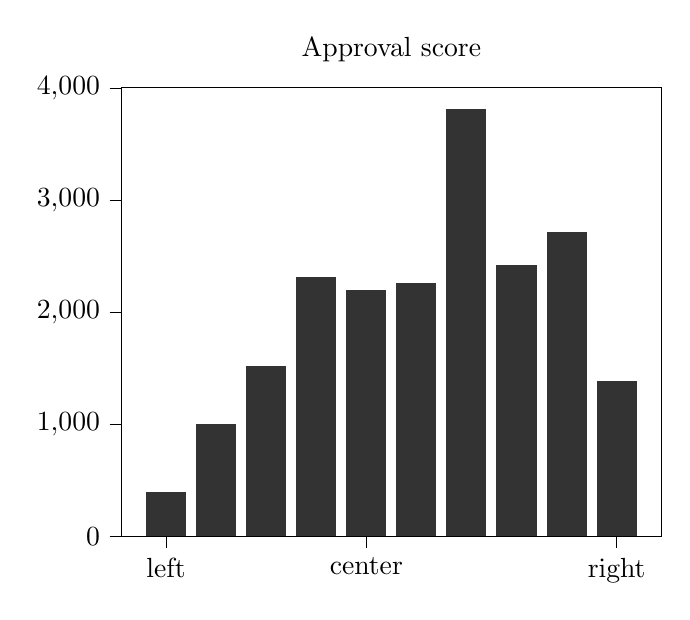
\begin{tikzpicture}

\definecolor{darkgray176}{RGB}{176,176,176}

\begin{axis}[
tick align=outside,
tick pos=left,
title={Approval score},
x grid style={darkgray176},
xmin=-0.89, xmax=9.89,
xtick style={color=black},
xtick={0,4,9},
xticklabels={left,center,right},
y grid style={darkgray176},
ymin=0, ymax=4000.5,
ytick style={color=black}
]
\draw[draw=none,fill=black,fill opacity=0.8] (axis cs:-0.4,0) rectangle (axis cs:0.4,395);
\draw[draw=none,fill=black,fill opacity=0.8] (axis cs:0.6,0) rectangle (axis cs:1.4,999);
\draw[draw=none,fill=black,fill opacity=0.8] (axis cs:1.6,0) rectangle (axis cs:2.4,1516);
\draw[draw=none,fill=black,fill opacity=0.8] (axis cs:2.6,0) rectangle (axis cs:3.4,2311);
\draw[draw=none,fill=black,fill opacity=0.8] (axis cs:3.6,0) rectangle (axis cs:4.4,2193);
\draw[draw=none,fill=black,fill opacity=0.8] (axis cs:4.6,0) rectangle (axis cs:5.4,2255);
\draw[draw=none,fill=black,fill opacity=0.8] (axis cs:5.6,0) rectangle (axis cs:6.4,3810);
\draw[draw=none,fill=black,fill opacity=0.8] (axis cs:6.6,0) rectangle (axis cs:7.4,2421);
\draw[draw=none,fill=black,fill opacity=0.8] (axis cs:7.6,0) rectangle (axis cs:8.4,2711);
\draw[draw=none,fill=black,fill opacity=0.8] (axis cs:8.6,0) rectangle (axis cs:9.4,1389);
\end{axis}

\end{tikzpicture}
